\documentclass[pdflatex,sn-mathphys-num]{sn-jnl}

\usepackage{graphicx}
\usepackage{multirow}
\usepackage{amsmath,amssymb,amsfonts}
\usepackage{booktabs}

\begin{document}

\title[Springer Nature Test Article]{A Springer Nature Journal Article with Figures}

\author*[1]{\fnm{Paper} \sur{Desk}}\email{test@example.com}
\author[1,2]{\fnm{Second} \sur{Author}}\email{second@example.com}

\affil*[1]{\orgdiv{Department of Testing}, \orgname{Example University}, \orgaddress{\city{Example City}, \country{Exampleland}}}
\affil[2]{\orgname{Example Institute}, \orgaddress{\city{Other City}, \country{Exampleland}}}

\abstract{This article checks the Springer Nature \texttt{sn-jnl} class with raster figures,
a table, equations and a numbered bibliography.}

\keywords{LaTeX, Springer Nature, figures, testing}

\maketitle

\section{Introduction}\label{sec:intro}
Figure~\ref{fig:results} shows a bar chart and Figure~\ref{fig:sample} a generated image.
Shannon's work~\cite{shannon1948} and Knuth's book~\cite{knuth1984} are cited here.

\begin{figure}[h]
  \centering
  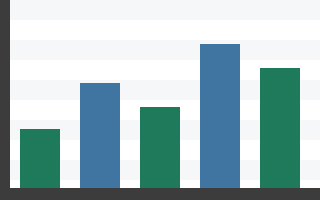
\includegraphics[width=0.6\textwidth]{figures/results.png}
  \caption{Results shown as a bar chart (PNG figure).}\label{fig:results}
\end{figure}

\section{Method}\label{sec:method}
\begin{equation}
  H(X) = -\sum_{i=1}^{n} p_i \log_2 p_i
  \label{eq:entropy}
\end{equation}
Entropy~\eqref{eq:entropy} is used in Table~\ref{tab:values}.

\begin{table}[h]
  \caption{Example values.}\label{tab:values}
  \begin{tabular}{@{}lcc@{}}
    \toprule
    Case & $p$ & $H$ (bits) \\
    \midrule
    Fair coin   & 0.5 & 1.000 \\
    Biased coin & 0.9 & 0.469 \\
    \botrule
  \end{tabular}
\end{table}

\begin{figure}[h]
  \centering
  
\includegraphics[width=0.45\textwidth]{figures/sample.png}
  \caption{A generated sample image.}\label{fig:sample}
\end{figure}

\section{Conclusion}\label{sec:conclusion}
The figures, table and references above should all appear in the PDF.

\backmatter
\bmhead{Acknowledgements}
Thanks to the PaperDesk test suite.

\bibliography{sn-bibliography}

\end{document}
